\title{B Trees and B+ Trees in Interactive HTML5}
\author{
  John Gunderman and Kenneth Watka \\
  Case Western Reserve University\\
}
\date{\today}

\maketitle

\begin{abstract}
B Trees and B+ Trees are tree structures used for the efficient
storage and retrieval of key/value pairs. Both data structures are
heavily used in the field of Computer Science for a wide variety of
applications. In this project, we devise a new learning tool for
students to better understand the operations performed by B and B+ Trees.
\end{abstract}

\setcounter{tocdepth}{1}
\tableofcontents
\vspace{.5in}
% No section for the introduction?

Our project aims to create a visualization of B and B+ trees using HTML5
technologies such as the \textit{canvas} element and Javascript. The user will open the
webpage and be presented with an interface that allows them to insert, delete
and search through these structures, with a visualization of how the
operations are performed.

B and B+ Trees are important data structures to be familiar with for
anyone working in the field of Computer Science. While literature on
the data structures is extensive, there does not exist a good
interactive visualization tool for observing the data structures in
action. The few tools that do exist for this purpose are somewhat old
and are written in Java. We found HTML5 and Javascript to be a much
more appealing and accessible language in today's web-connected world,
and thus chose to bring these old visualization tools into the modern day.


\section{Approach}

\subsection{B and B+ Backend}
Our apporach to creating the backend which would handle the structure
of the trees and their contents was fairly straight forward.  We had
access to well defined rules that define B and B+ trees so designing
the general structure of the trees was simple enough.  However, since
our intent was for the web interface to ba able to actively switch
between B and B+ tree representations we had to factor in as much
shared resources as we could to assist in the process of switching
between the two tree types.  Conveniently, B and B+ trees are fairly
similar, so it did not take much extra effort to make much of the
trees structure shared.  Specficially, both tree types utilize the
same node/block object we have created.  While the nodes have some
properties unique to either type of tree, which comes at a slight
memory cost, it makes it easier to switch back and forth.  We also
keep a master list of all values in the tree at any given time.  This
master list is the primary element that allows us to switch between
tree structures.  Whenever we want to switch, we simply copy the
element list, change the tree type, and then insert every value into
the tree, in the same order they had been inserted into the previous
tree.  It should be noted that this method could result in getting a
different tree if you switched from B tree to B+ and back again, or
vice versa.  this is because we do not execute all opperations that
occurred on the previous tree, just insertions of values that were in
it, so any imperfect organization caused by deletion could be cleaned
up by switching back and orth between tree structures.  While
structurally the trees have various commonalities, the methods of
insertion, deletion, and searching the trees still had to remain
completely separate due to the subtly differences in the tree
structures.

\subsection{HTML5 Frontend}
Due to the dynamic nature of the content we needed to display to the
user, we decided to use the HTML5 \texttt{canvas} element. With the
\texttt{canvas} element, it is possible to draw things directly on the
screen. However, the \texttt{canvas} element is quite low level in
its functionality. In order to utilize higher order abstractions, we
utilized a library called \textit{Kinetic.js}. This library allowed us
to specify groups of shapes which would be considered as a consistent
whole when moving across the screen. From this we could construct node
and edge objects which would be consistent throughout the modelling
process.

User input occurs through the use of text boxes and buttons directly
underneath the \texttt{canvas} display. These buttons are labeled with
the different possible actions: insert, delete, and search. By
inputting a value into the associated text box, and pressing the
button, the user initiates a modification to the tree.

%% \begin{figure}[htp]
%% \centering
%% 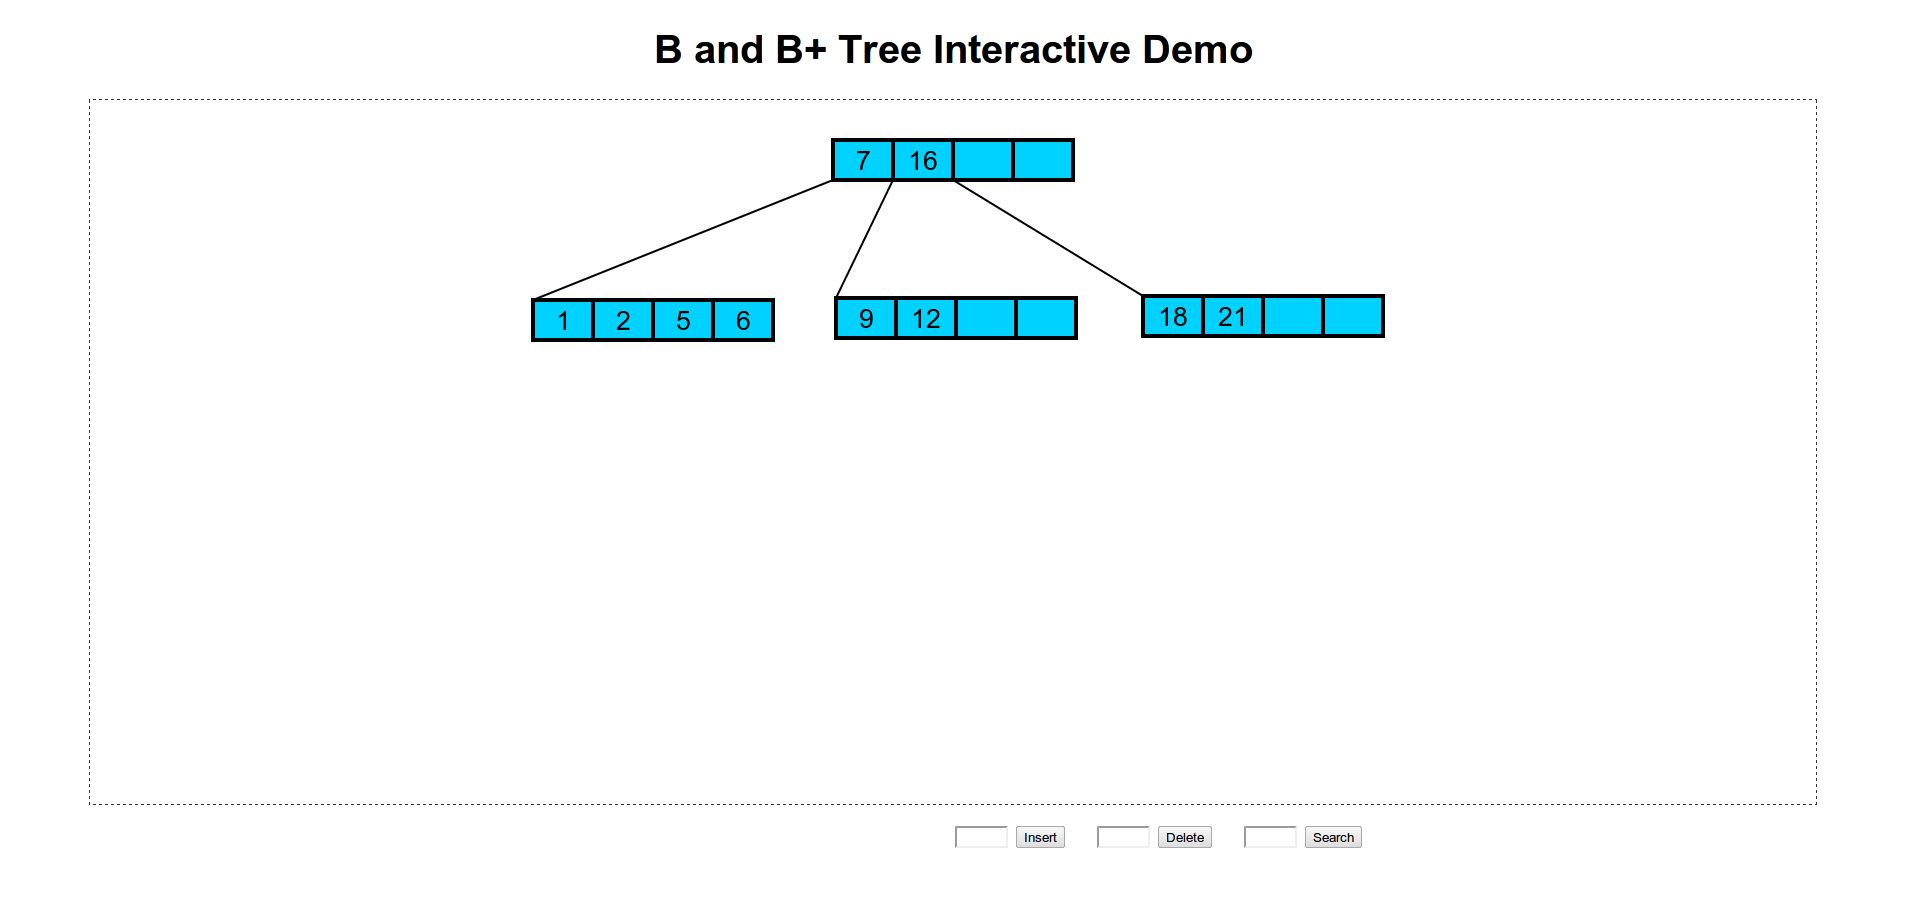
\includegraphics[scale=0.25]{images/Interface.png}
%% \caption{The user interface of our project}
%% \label{UI}
%% \end{figure}

\section{Algorithms}

% kenny, put a section here about B+ algorithms

The UI portion of this project requires a sizable amount of
algorithmic work. The most difficult factor is the development of a
node layout algorithm that prevents node overlap, while also giving an
ideal spacing between the nodes in the tree. This is especially
important as the size of the tree grows.

A popular method for solving this problem is the use of the
force-based algorithm. This algorithm works well for spreading nodes
out over 2 or 3 dimensional space. However, it does not take into
account the movement limitations that are imposed in a B+
tree. Namely, the nodes in a B+ tree can only move horizontally except
for in the case of a node split or join. This limitation requires
non-trivial modifications to the algorithm.

A secondary issue with the use of force-based algorithms is that they
have a running time of O$(n^3)$. This 



\section{Changes}



\section{Future Work}

Future changes we would like to make to our project would include a
hefty redesign for some of the tre structure algorithms, specifically
the deletion methods.  Our current deletion algorithms do a complete
restructuring of the tree when we encounter an underflow because of
deletion.  This method is convenient for reducing lines of code, but
can become very costly for large trees.  As such in the future we hope
to be able to implement the more common method for handling deletion
that results in underflow, which is to then cascade upward, merge with
or borrowing from sibling nodes.  In the general case this method
would prove to have better performance, having a deletion time of
O(log n) as oppposed to our current method which has a deletion time
of O(n log n).  Part of the reason we didn't not do the standard
method of deletion initially was because of some of the limitation fo
Javascript.  Javascript lacks easy to use pointers, which made things
a bit harder when trying to keep track for each node/block, what it's
children and parent were.  As such we could not find a reasonable
method of linking sibling nodes which would be necessary for efficient
implementation of standard method of handling underflow by borrowing
or merging with siblings.  We'd also like to better organize the
modularization of our insertion methods, while they work, and run in
time O(log n) the code itself is a bit disorganized making it hard to
read through if you were trying to go through it manually to verify
correctness.

Visually, it would also be a nice addition if we could provide step by
step animation of how values, or a search is moving through the tree
to provide a better means of understanding exactly what is occurring
during various search, insertion, or deletion queries.  A simple
textual output could suffice if it explicitly stated things like:
"Key 3 removed from node X"
"Node X borrowed values a,b from node Y to cover underflow"
...
"Key 6 inserted into Node X"
"Node X split into Nodes Y, with values a,b, and Z, with values c,d"
etc.

This atleast would allow the user to follow along with the action step
by step, even if they could not see if visually animated.

\section{Conclusion}

Our project successfully met the goals we set out to accomplish when
we began this project. The user can successfully insert, delete, and
search for values in the B or B+ Tree. At each action, the user
recieves a visualization of the new tree state.

In the process of develooping this project, we came across more great
ideas for features we could develop. These are detailed above, in the
\textit{Future Work} section.


